% $Header: /Users/josph/Documents/LaTeX/beamer/solutions/generic-talks/generic-ornate-15min-45min.en.tex,v 90e850259b8b 2007/01/28 20:48:30 tantau $

\PassOptionsToPackage{subsection=false}{beamerouterthememiniframes} % prevent subsection bar in outer theme
\documentclass{beamer}
\usepackage{attrib}
\usepackage{xstring}
\includeonlylecture{02}
\mode<presentation>
{
  \usetheme{Szeged}
  \setbeamercovered{transparent}
}

\usepackage[english]{babel}
\usepackage[latin1]{inputenc}
\usepackage{times}
\usepackage[T1]{fontenc}
\usepackage{remreset}% tiny package containing just the \@removefromreset command

%% Get the points on the presentation without subsections
\makeatletter
\@removefromreset{subsection}{section}
\makeatother
\setcounter{subsection}{1}

%%%%%%%%%%%%%%
% Custom macros and environments
\newenvironment{goals}
{
\newcommand{\goal}{\item[--]}
\begin{frame}[fragile,environment=goals]
\frametitle{Goals}
\begin{itemize}	
}
{\end{itemize}
\end{frame}
}

\newcommand{\versehighlight}[2]{
\def\v{#2}
\def\x{#1}
\expandarg
\StrSubstitute{\x}{\v}{\alert{\v}}
}

\newcommand{\keyverse}{
31 Behold, the days are coming, declares the Lord, when I will make a new covenant with the house of Israel and the house of Judah, 32 not like the covenant that I made with their fathers on the day when I took them by the hand to bring them out of the land of Egypt, my covenant that they broke, though I was their husband, declares the Lord. 33 For this is the covenant that I will make with the house of Israel after those days, declares the Lord: I will put my law within them, and I will write it on their hearts. And I will be their God, and they shall be my people.}

\newcommand{\keyversehiglight}[1]{
\versehighlight{\keyverse}{#1}
}

%%%%%%%%%%%%%%
\title[] % (optional, use only with long paper titles)
{``For They Shall All Know Me''}

\subtitle
{Developing a New Covenant Relationship with God} % (optional)

%\author[Author, Another] % (optional, use only with lots of authors)
%{F.~Author\inst{1} \and S.~Another\inst{2}}
% - Use the \inst{?} command only if the authors have different
%   affiliation.

%\institute[Universities of Somewhere and Elsewhere] % (optional, but mostly needed)
%{
%  \inst{1}%
  %Department of Computer Science\\
  %University of Somewhere
  %\and
  %\inst{2}%
  %Department of Theoretical Philosophy\\
  %University of Elsewhere}
%% - Use the \inst command only if there are several affiliations.
%% - Keep it simple, no one is interested in your street address.

\date[Sun. AM] % (optional)
{Spring 2016 / Sunday AM Bible Study}

\subject{Sunday morning classes Walnut Street Church of Christ}
% This is only inserted into the PDF information catalog. Can be left
% out. 



% If you have a file called "university-logo-filename.xxx", where xxx
% is a graphic format that can be processed by latex or pdflatex,
% resp., then you can add a logo as follows:

% \pgfdeclareimage[height=0.5cm]{university-logo}{university-logo-filename}
% \logo{\pgfuseimage{university-logo}}



% Delete this, if you do not want the table of contents to pop up at
% the beginning of each subsection:
\AtBeginSubsection[]
{
  \begin{frame}<beamer>{Outline}
    \tableofcontents[currentsection,currentsubsection]
  \end{frame}
}

% When having one big beamer document for the entire course you can customize the output for each class.
\AtBeginLecture{
\frame{\Large \insertlecture}
\begin{frame}{Outline}
  \tableofcontents
  % You might wish to add the option [pausesections]
\end{frame}
}
% If you wish to uncover everything in a step-wise fashion, uncomment
% the following command: 

%\beamerdefaultoverlayspecification{<+->}


\begin{document}

\begin{frame}
  \titlepage
\end{frame}

\lecture{Introduction}{01-Introduction}
% - Exactly two or three sections (other than the summary).
% - At *most* three subsections per section.
% - Talk about 30s to 2min per frame. So there should be between about
%   15 and 30 frames, all told.

\section{Introduction}

\begin{goals}
\goal Become familiar with the class theme, key passage, and class objectives.
\goal Understand how each subsequent lesson fits into the class objectives.
\goal Do an initial evaluation of how relationship-focused your religion is.
\end{goals}

\begin{frame}
\begin{quote}
31 Behold, the days are coming, declares the Lord, when I will make a new covenant with the house of Israel and the house of Judah, 32 not like the covenant that I made with their fathers on the day when I took them by the hand to bring them out of the land of Egypt, my covenant that they broke, though I was their husband, declares the Lord. 33 For this is the covenant that I will make with the house of Israel after those days, declares the Lord: I will put my law within them, and I will write it on their hearts. And I will be their God, and they shall be my people. \attrib{Jeremiah 31:31-33}
\end{quote}
\end{frame}

%\begin{discussion}
%\dsubsec{Introduction}{900-905}{5}
%
%This lesson is about who God is.
%
%\bvs{Genesis}{(17:1-8)} God's first covenant with Abraham says that he will be his God.
%
%\dsubsec{Who is God?}{905-915}{10}
%
	%\bvs{Psalms}{(8:1-9)} It's amazing that God is is mindful of us.
%
%\dsubsec{How we come to know about God}{915-925}{10}
%
	%\bvs{Ecclesiastes}{(3:11)} Eternity in the heart of man
%
  %\bvs{Hebrews}{(1:1-2)} Fathers by the prophets, today His son
	%
	%By extension His Word.
%
%\dsubsec{What does that mean for me?}{925-940}{15}
%
	%\bvs{Luke}{(4:1-13)} Having a God gives you an anchor. 
	%
	%\bvs{Luke}{(14:25-27)} Love God and you will live.
%
%\dsubsec{Review}{940-945}{5}
%\end{discussion}

%\begin{frame}{Class Theme}{Subtitles are optional.}
  %% - A title should summarize the slide in an understandable fashion
  %%   for anyone how does not follow everything on the slide itself.
%
  %\begin{itemize}
  %\item
    %Use \texttt{itemize} a lot.
  %\item
    %Use very short sentences or short phrases.
  %\end{itemize}
%\end{frame}
%\begin{frame}{Lesson Motivation}{Subtitles are optional.}
  %% - A title should summarize the slide in an understandable fashion
  %%   for anyone how does not follow everything on the slide itself.
%
  %\begin{itemize}
  %\item
    %Use \texttt{itemize} a lot.
  %\item
    %Use very short sentences or short phrases.
  %\end{itemize}
%\end{frame}
%\begin{frame}{Lesson Objectives}{Subtitles are optional.}
  %% - A title should summarize the slide in an understandable fashion
  %%   for anyone how does not follow everything on the slide itself.
%
  %\begin{itemize}
  %\item
    %Use \texttt{itemize} a lot.
  %\item
    %Use very short sentences or short phrases.
  %\end{itemize}
%\end{frame}
%\section{Point1}
%\section{Point2}
%\section{Point3}
%\subsection[Objectives]{Theme}
%\subsection[Short First Subsection Name]{First Subsection Name}
%
%\begin{frame}{Make Titles Informative. Use Uppercase Letters.}{Subtitles are optional.}
  %% - A title should summarize the slide in an understandable fashion
  %%   for anyone how does not follow everything on the slide itself.
%
  %\begin{itemize}
  %\item
    %Use \texttt{itemize} a lot.
  %\item
    %Use very short sentences or short phrases.
  %\end{itemize}
%\end{frame}
%
%\begin{frame}{Make Titles Informative.}
%
  %You can create overlays\dots
  %\begin{itemize}
  %\item using the \texttt{pause} command:
    %\begin{itemize}
    %\item
      %First item.
      %\pause
    %\item    
      %Second item.
    %\end{itemize}
  %\item
    %using overlay specifications:
    %\begin{itemize}
    %\item<3->
      %First item.
    %\item<4->
      %Second item.
    %\end{itemize}
  %\item
    %using the general \texttt{uncover} command:
    %\begin{itemize}
      %\uncover<5->{\item
        %First item.}
      %\uncover<6->{\item
        %Second item.}
    %\end{itemize}
  %\end{itemize}
%\end{frame}
%
%
%\subsection{Second Subsection}
%
%\begin{frame}{Make Titles Informative.}
%\end{frame}
%
%\begin{frame}{Make Titles Informative.}
%\end{frame}
%
%
%
%\section*{Summary}
%
%\begin{frame}{Summary}
%
  %% Keep the summary *very short*.
  %\begin{itemize}
  %\item
    %The \alert{first main message} of your talk in one or two lines.
  %\item
    %The \alert{second main message} of your talk in one or two lines.
  %\item
    %Perhaps a \alert{third message}, but not more than that.
  %\end{itemize}
  %
  %% The following outlook is optional.
  %\vskip0pt plus.5fill
  %\begin{itemize}
  %\item
    %Outlook
    %\begin{itemize}
    %\item
      %Something you haven't solved.
    %\item
      %Something else you haven't solved.
    %\end{itemize}
  %\end{itemize}
%\end{frame}


\lecture{2. I will be their God}{02}

\section*{Introduction}

\begin{frame}
\frametitle{Texas is my state}
	\begin{center}
	
\includegraphics[width=.9\textwidth]{figures/texas.jpg}
	\end{center}
\note{09:30}
\note[item]{I, like most Texans, am proud where I come from.}
\note[item]{Texans are taught that their state is simply better than any other state (or country).}
\note[item]{God wants us to think that way about Him -- that He is simply better.}
\note[item]{He is the only one that deserves our loyalty.}
\note[item]{He wants His team to be the only team we play for.}
\end{frame}

\begin{frame}
\frametitle{God wants a relationship with people}
\framesubtitle{Jeremiah 31:31-34}
	\keyversehiglight{I will be their God}
	\note{09:32}
	\note[item]{In our class we're trying to establish, from the Bible, the idea that God 
wants a relationship with people.}
	\note[item]{We're using Jeremiah 31:31-34 as a means of focusing that study.}
	\note[item]{Jeremiah 31:31-34 is one of the most important passages in the Bible, because it provides a connection between the old covenant and the new covenant, and talks about the close, special relationship that God's chosen people have with Him.  Under the old covenant, those people were the Israelites.  Under the New Covenant, those special people are all Christians.}
	\note[item]{\emph{Read it}}
	\note[item]{Today we'll be talking about how God wants to be the only God in our lives.}
\end{frame}

\begin{goals}
\goal Consider who God is, and consider how He is similar and different from man.
\goal Explore the different ways God has revealed himself to man.
\goal Think about ways to improve my perspective on who God is.

\note{09:33}
\note[item]{Examine why God is worthy of our loyalty.}
\note[item]{Examine how we learn about God's greatness.}
\note[item]{Considering how we can increase our devotion to God.}
\end{goals}

\section{I will be your God}

\begin{frame}
\frametitle{I will be your God}
\framesubtitle{Gen 17:1-8}
\begin{columns}[T]
	\begin{column}{0.4\textwidth}
		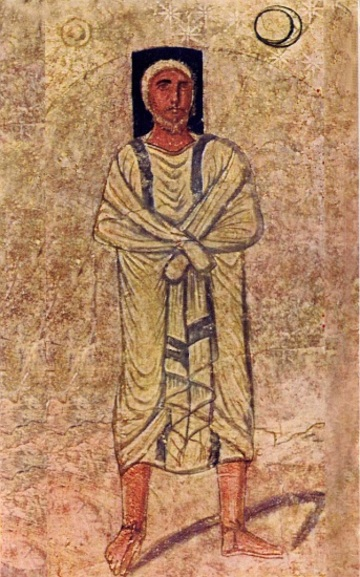
\includegraphics[height=0.8\textheight]{figures/abrahamDuraEuropos.jpg}
	\end{column}
	\begin{column}{0.6\textwidth}
		``And I will give you and to your offspring after you the land of your sojournings, all the land of Canaan, for an everlasting possession, and \\\alert{I will be their God}.'' -- Genesis 17:8
	\end{column}
\end{columns}

\note{09:35}
\note[item]{God recounts his 3-fold promise to Abraham: land, nation, seed (if you count ``kings shall come from you'')}.
\note[item]{Part or all of these promises are repeated at various times in Abraham's life (Gen 12, 13, 15, 17, 22)}
\note[item]{The first occurrence of the phrase `I will be their God' is in God's promise to Abraham.}
\note[item]{Fresco pictured here is one of the earliest depictions of a Bible narrative.  It depicts Abraham and God's promises to Him.  It is from the Dura-Europos synagogue 244 AD  70\% of the city has been destroyed during the Syrian civil war.}
\note[item]{When does God mean when he says `I will be their God'? \emph{Abraham had many `gods' to choose from, but God wanted Abraham to love only Him.}}
\note[item]{vs.1-2 Because God is mighty, he had to put a condition on His covenant with Abraham -- be blameless.}
\end{frame}

\begin{frame}
\frametitle{`I will be their God' through the Bible}
\begin{columns}[T]
	\begin{column}{0.45\textwidth}
		`I will be their God'\\{\footnotesize Gen. 17:8, Jer. 24:7, Jer. 31:33\\Jer. 32:36, Jer. 32:38, Ez. 11:20\\Ez. 37:15, Ez. 37:23, Ez. 37:27\\Zech. 8:8, 2 Cor. 6:16, Heb. 8:10}\\~\\
		`I will be your God'\\{\footnotesize Ex. 6:7, Jer. 7:23, Jer. 11:4\\Jer. 30:2, Ez. 36:28}\\~\\
	\end{column}
	\begin{column}{0.55\textwidth}
			`the Lord your God'\\ 
			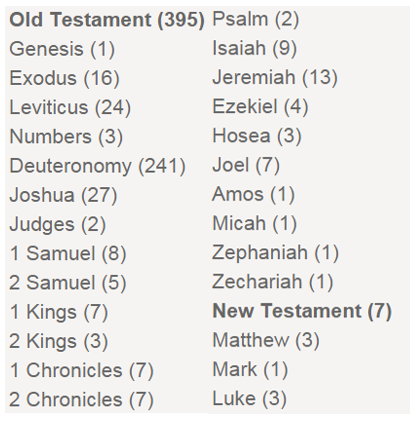
\includegraphics[width=1\columnwidth]{figures/theLordYourGodTwoColumn.png}
	\end{column}
\end{columns}

\note{09:38}
\note[item]{Last week, `your God', given to the Israelites as part of the Law of Moses (Ex. 6:1-9, Lev. 22:31-33).}
\note[item]{Clearly God thinks it's important that we view Him as the only God.}
\note[item]{It's not just that His people accept Him as the `true' God.  But as `their' God}
\end{frame}

\section{Who is God?}

\begin{frame}
\frametitle{God is majestic}
\framesubtitle{Psalm 8}
\begin{center}
	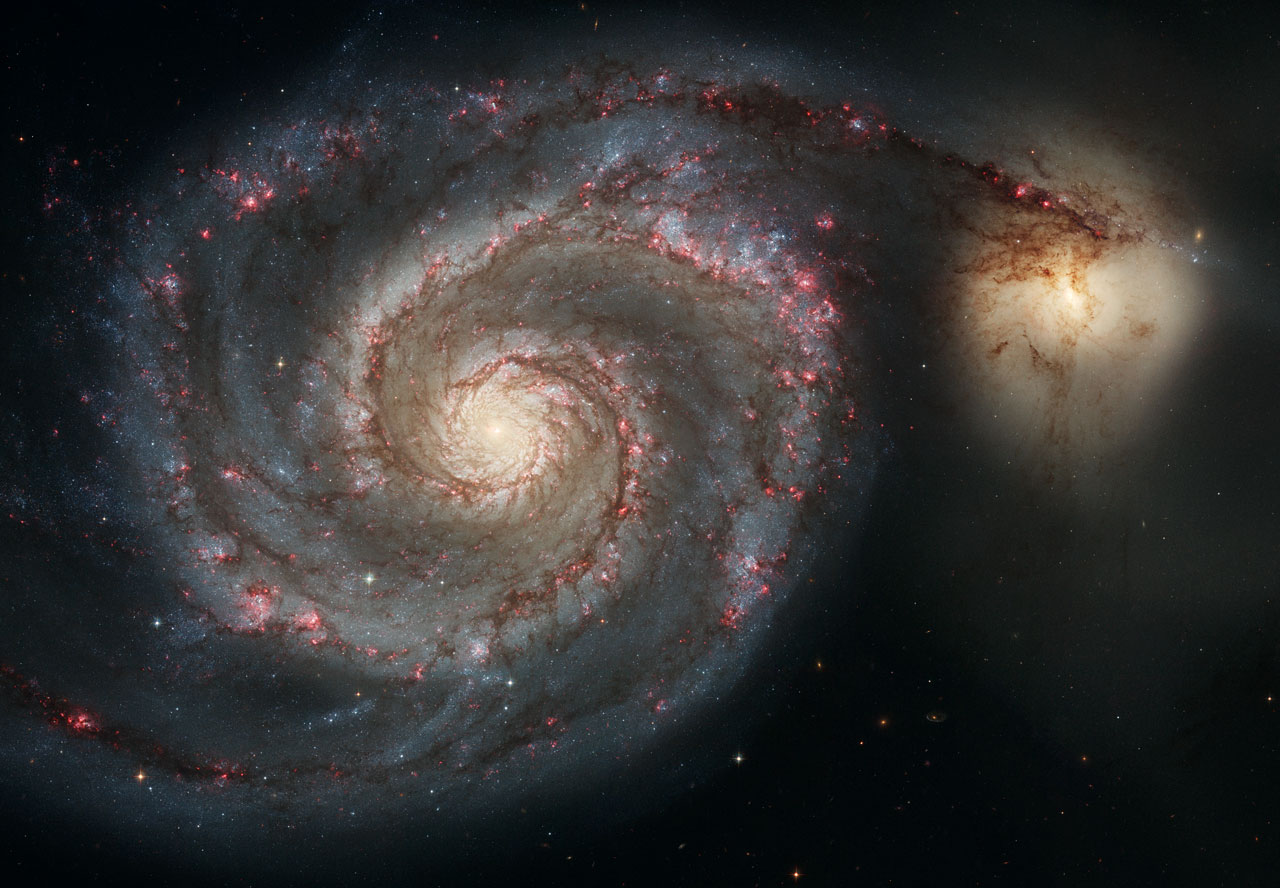
\includegraphics[width=0.85\textwidth]{figures/galaxy.jpg}\\
	{\footnotesize The Whirlpool galaxy as seen from the Hubble Space Telescope}
\end{center}

\note{09:40}
\note[item]{The Whirlpool galaxy is 60,000 LY across.  You can see it clearly with your own telescope.  Right below the handle of the big dipper.}
\note[item]{I'm small compared to God.}
\end{frame}

\begin{frame}
\frametitle{Man is not the source of God's greatness}
\framesubtitle{Psalm 8}
Out of the mouth of babes and sucklings hast thou perfected praise, because of thine enemies; that thou mightest put down the enemy and avenger.\hfill--Psalm 8:2 (LXX)\\~\\
15 But when the chief priests and the scribes saw the wonderful things that he did, and the children crying out in the temple, ``Hosanna to the Son of David!'' they were indignant, 16 and they said to him, ``Do you hear what these are saying?'' And Jesus said to them, ``Yes; have you never read,
\begin{quote}
`Out of the mouth of infants and nursing babies you have prepared praise'?
\end{quote}\\
\hfill-- Matt. 21:15-16 (ESV)
\normalsize

\note{09:41}
\note[item]{In context, Psalm 8:2 may refer to Israel, who followed the true God, being small and the surrounding nations being `great'.}
\note[item]{Jesus quotes Psalm 8:2 to remind the chief priests and scribes that they are not the source of His approval.}
\note[item]{It's important to remember that God is great, whether or not man accepts it.}
\end{frame}

\begin{frame}
\frametitle{God loves man and has blessed him.}
\framesubtitle{Psalm 8}
\begin{center}
	
\includegraphics[width=\textwidth]{figures/manLandscape.jpg}\\
	``The worst moment for the atheist is when he is really thankful and has nobody to thank.''
\end{center}

\note{09:45}
\note[item]{Man is not powerful like God is.}
\note[item]{Yet, He has made us special compared to all other creation}
\note[item]{Man is special and loved even when he rejects God.}
\note[item]{Quote is possibly attributed to Dante Gabriel Rossetti, a painter poet from the mid-19th century}
\end{frame}

\section{How we come to know about God}

\begin{frame}
\frametitle{Eternity is set in the heart of man}
\framesubtitle{Ecclesiastes 3:11}

\includegraphics[width=\textwidth]{figures/eternityInHeart.jpg}

\note{09:48}
\note[item]{God has always made Himself known to man}
\note[item]{What does the passage mean? \emph{Man innately understands the possibility that something could exist beyond his own world.}}
\note[item]{However God may have chosen to speak to us, He was always going to leverage that part of our being that understands there's something more to life.}
\note[item]{Romans 1 -- Creation speaks to an `un-caused cause', which should lead us to consider God.}

\end{frame}

\begin{frame}
	\frametitle{In the past, God spoke to the Fathers by the prophets}
	\framesubtitle{Hebrews 1:1-2}
	\begin{center}
	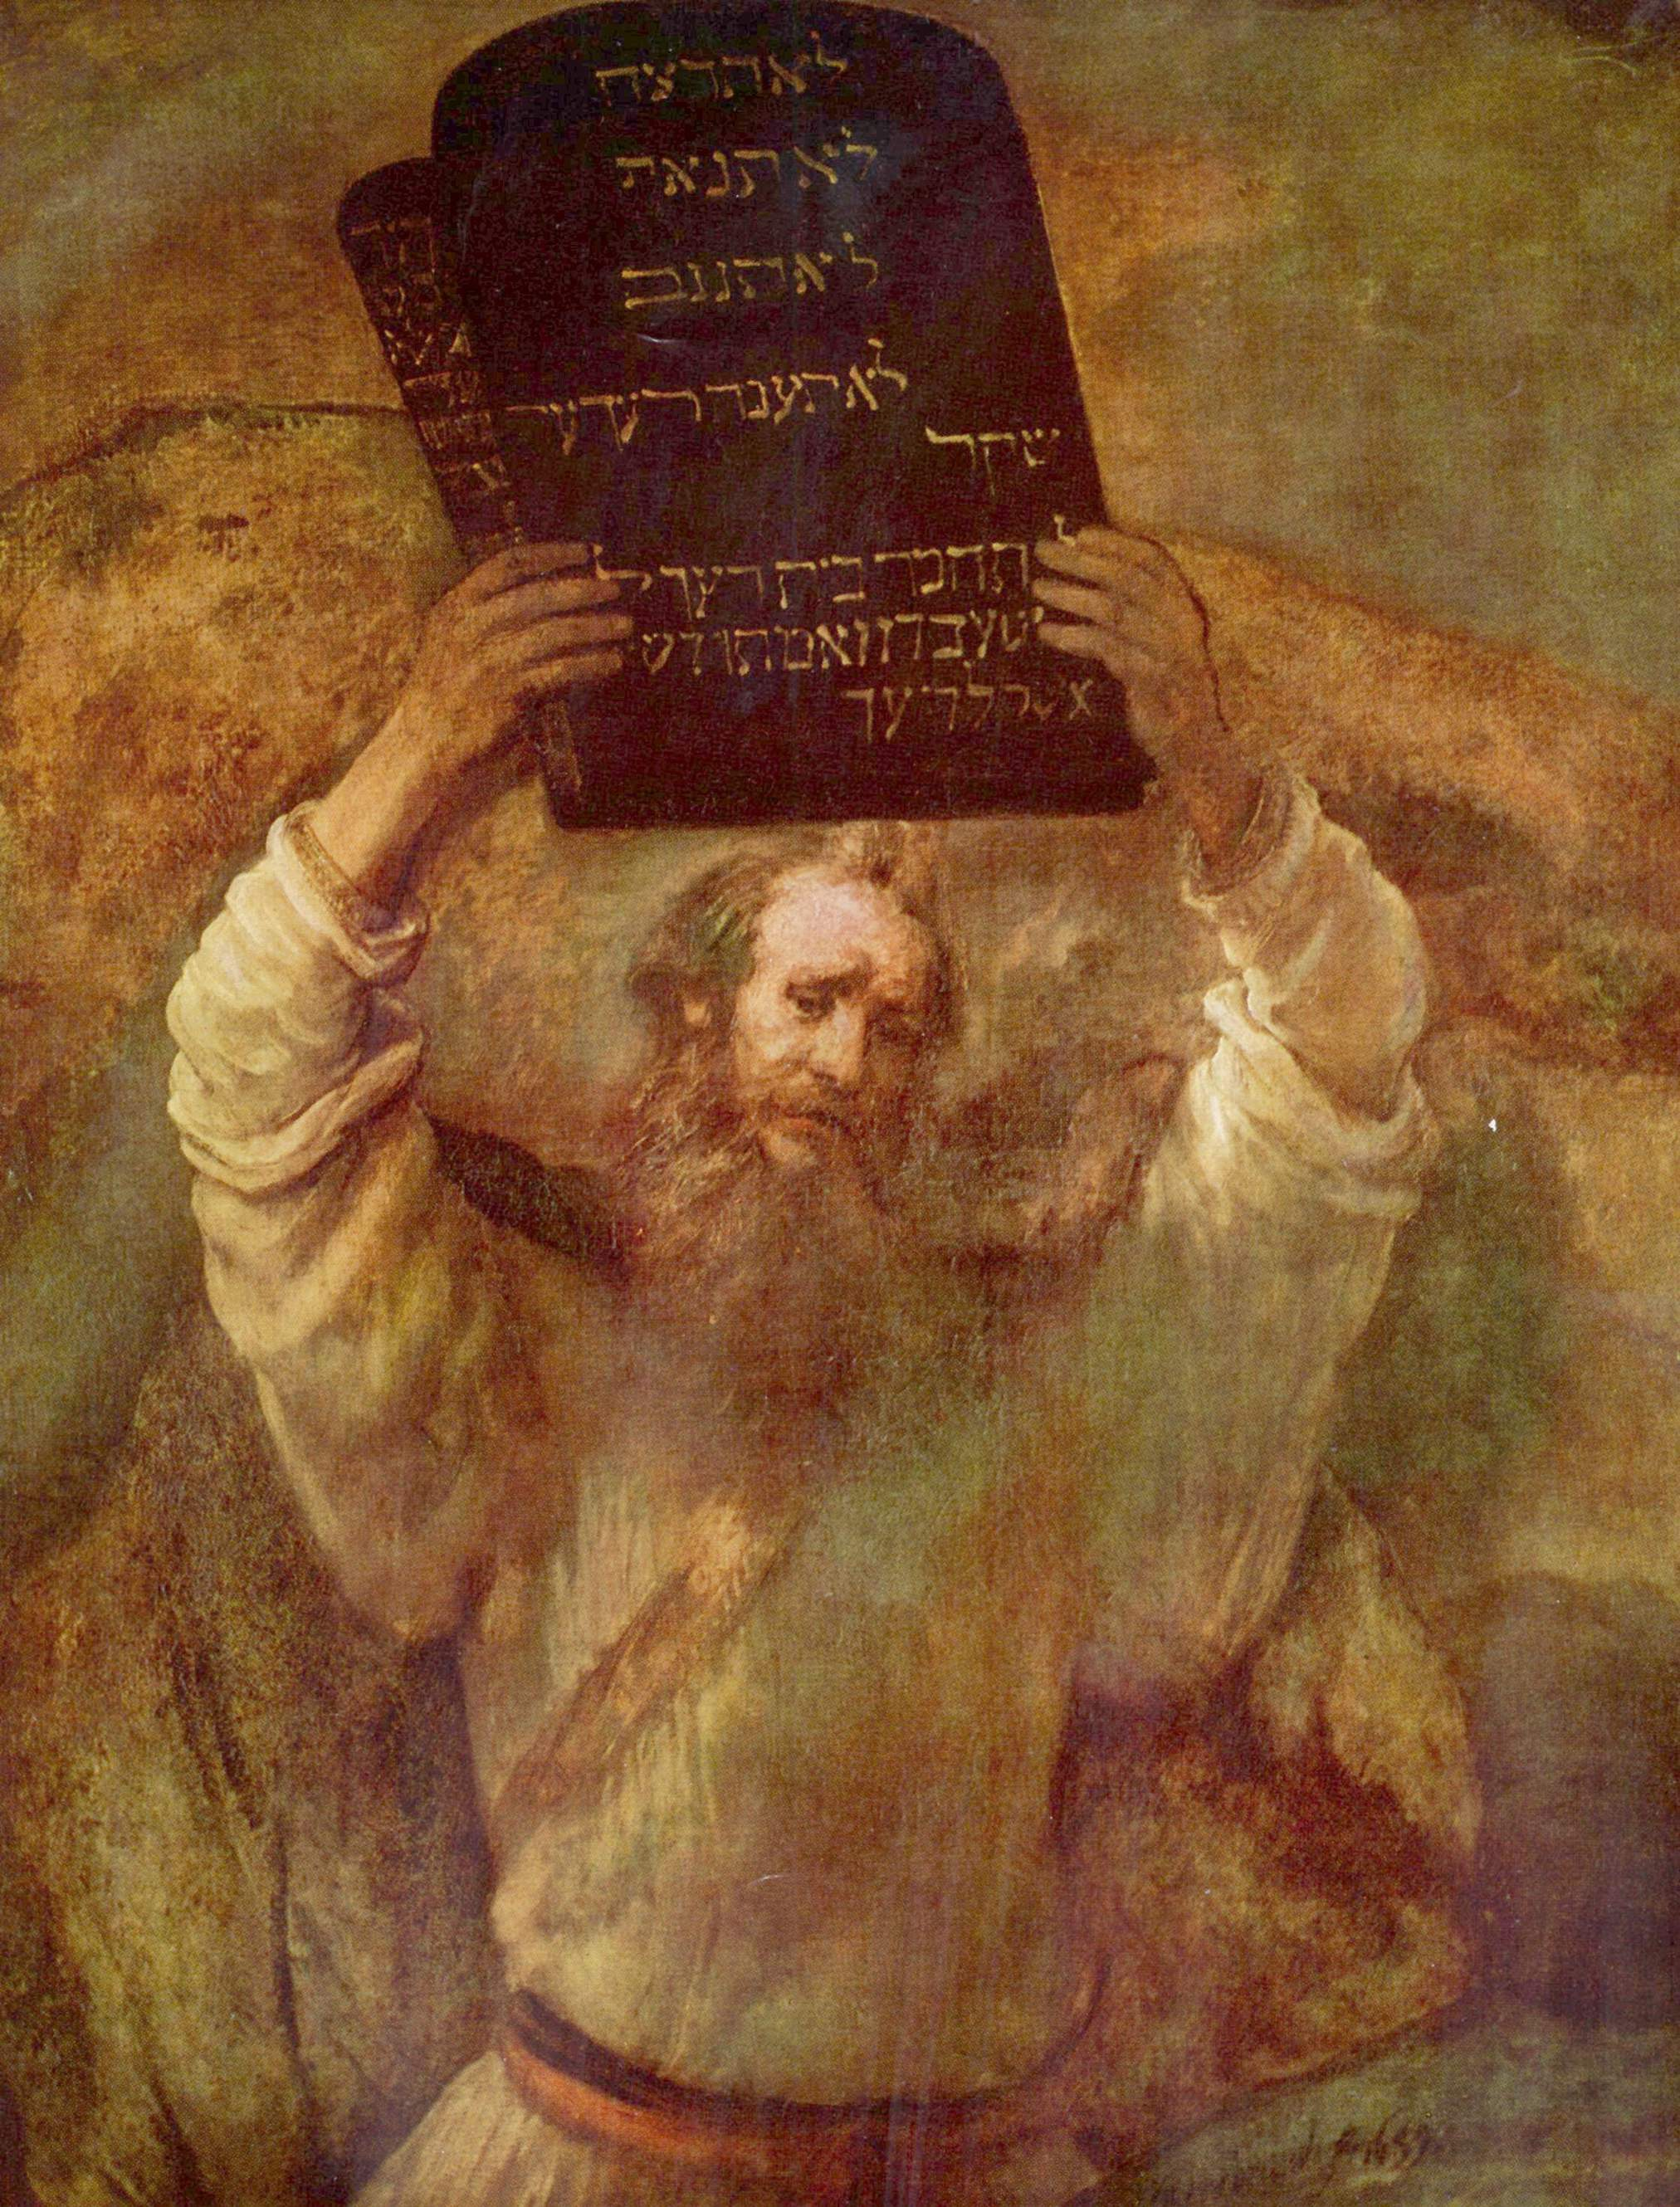
\includegraphics[height=0.8\textheight]{figures/mosesTenCommandments.jpg}
	\end{center}
	
	\note{09:50}
	\note[item]{The Israelites would have viewed Moses as the greatest prophet, the giver of God's Law.}
	\note[item]{Prophets would also include all those people we normally think of as prophets, whose main purpose was to plead for Israel to repent from wickedness.}
	\note[item]{The author leaves out the patriarchs. But, remember, he's just trying to make a point.}
	\note[item]{What's tough about learning from prophets? \emph{People don't have access to prophets all the time.  And, prophets just `tell' you what perfect faithfulness looks like.  They can't `show' you what perfect faithfulness looks like.}}
	\note[item]{Painting:Rembrandt}
\end{frame}

\begin{frame}
	\frametitle{Today, God speaks to us in His Son, Jesus}
	\framesubtitle{Hebrews 1:1-2}
	\begin{center}
	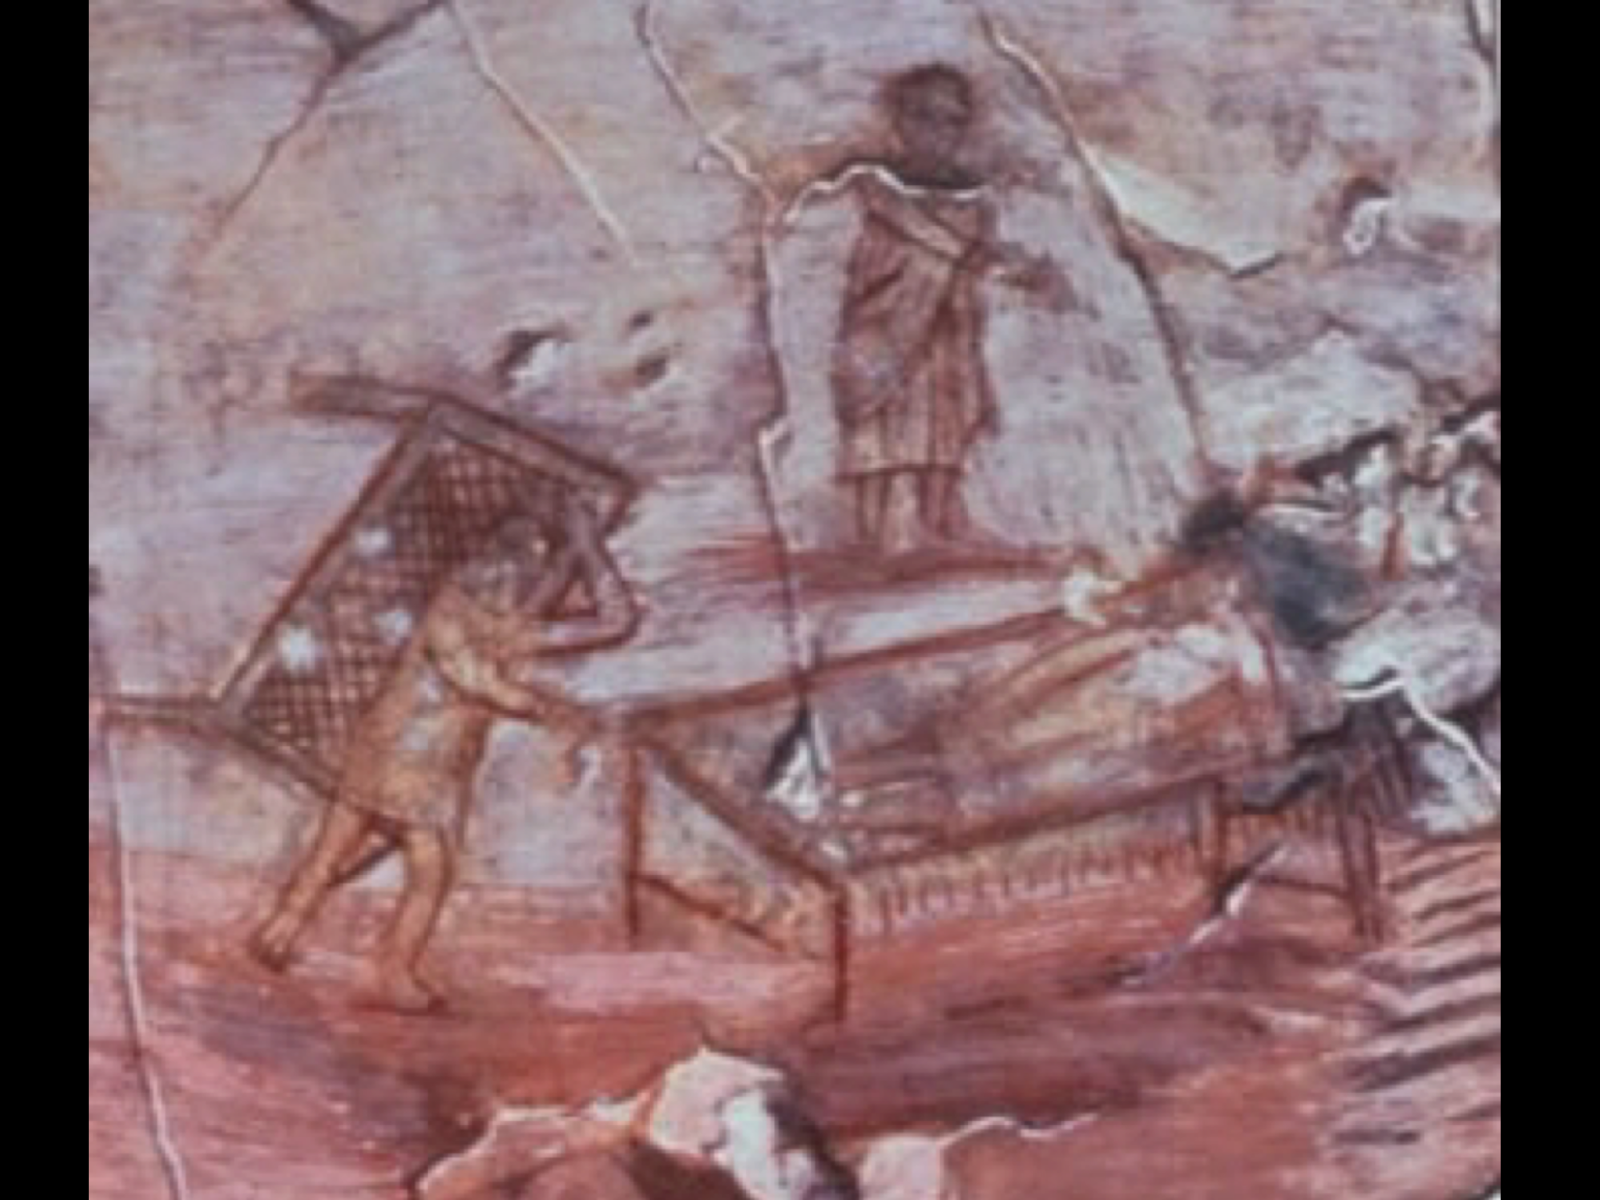
\includegraphics[height=0.8\textheight]{figures/jesusHealingParalytic.png}
	\end{center}
	
	\note{09:53}
	\note[item]{Speak means much more than simply teaching.}
	\note[item]{Jesus' life itself was God showing us how to live righteous.}
	\note[item]{God was under no obligation to do this.  He loved us.}
	\note[item]{But, even with Jesus, you only had direct access to his life if you lived in 1st century Palestine.}
	\note[item]{The fresco pictured is also from Dura-Europos (225AD), but a church instead of a synagogue.  It pictures Jesus healing the paralytic.  It's the earliest known depiction of Jesus.  In general, early Christians did not make images of Jesus.}
\end{frame}

\begin{frame}
	\frametitle{...And by extension His Word}
	\framesubtitle{Hebrews 1:1-2}
	\begin{center}
	
\includegraphics[width=\textheight]{figures/godSpeaksThroughTheWord.jpg}
	\end{center}
	
	\note{09:57}
	\note[item]{God has always shown Himself to man, but never more easily and more clearly than today}
	\note[item]{The Bible doesn't change through time.}
	\note[item]{The Bible is easily available for most people.}
	\note[item]{God makes himself `our God' when we read His word, understand it, and believe it}.
\end{frame}

\section{What does that mean for me?}

\begin{frame}
	\frametitle{God gives you moral anchor}
	\framesubtitle{Luke 4:1-13}
	\begin{columns}
	\begin{column}{0.5\textwidth}
	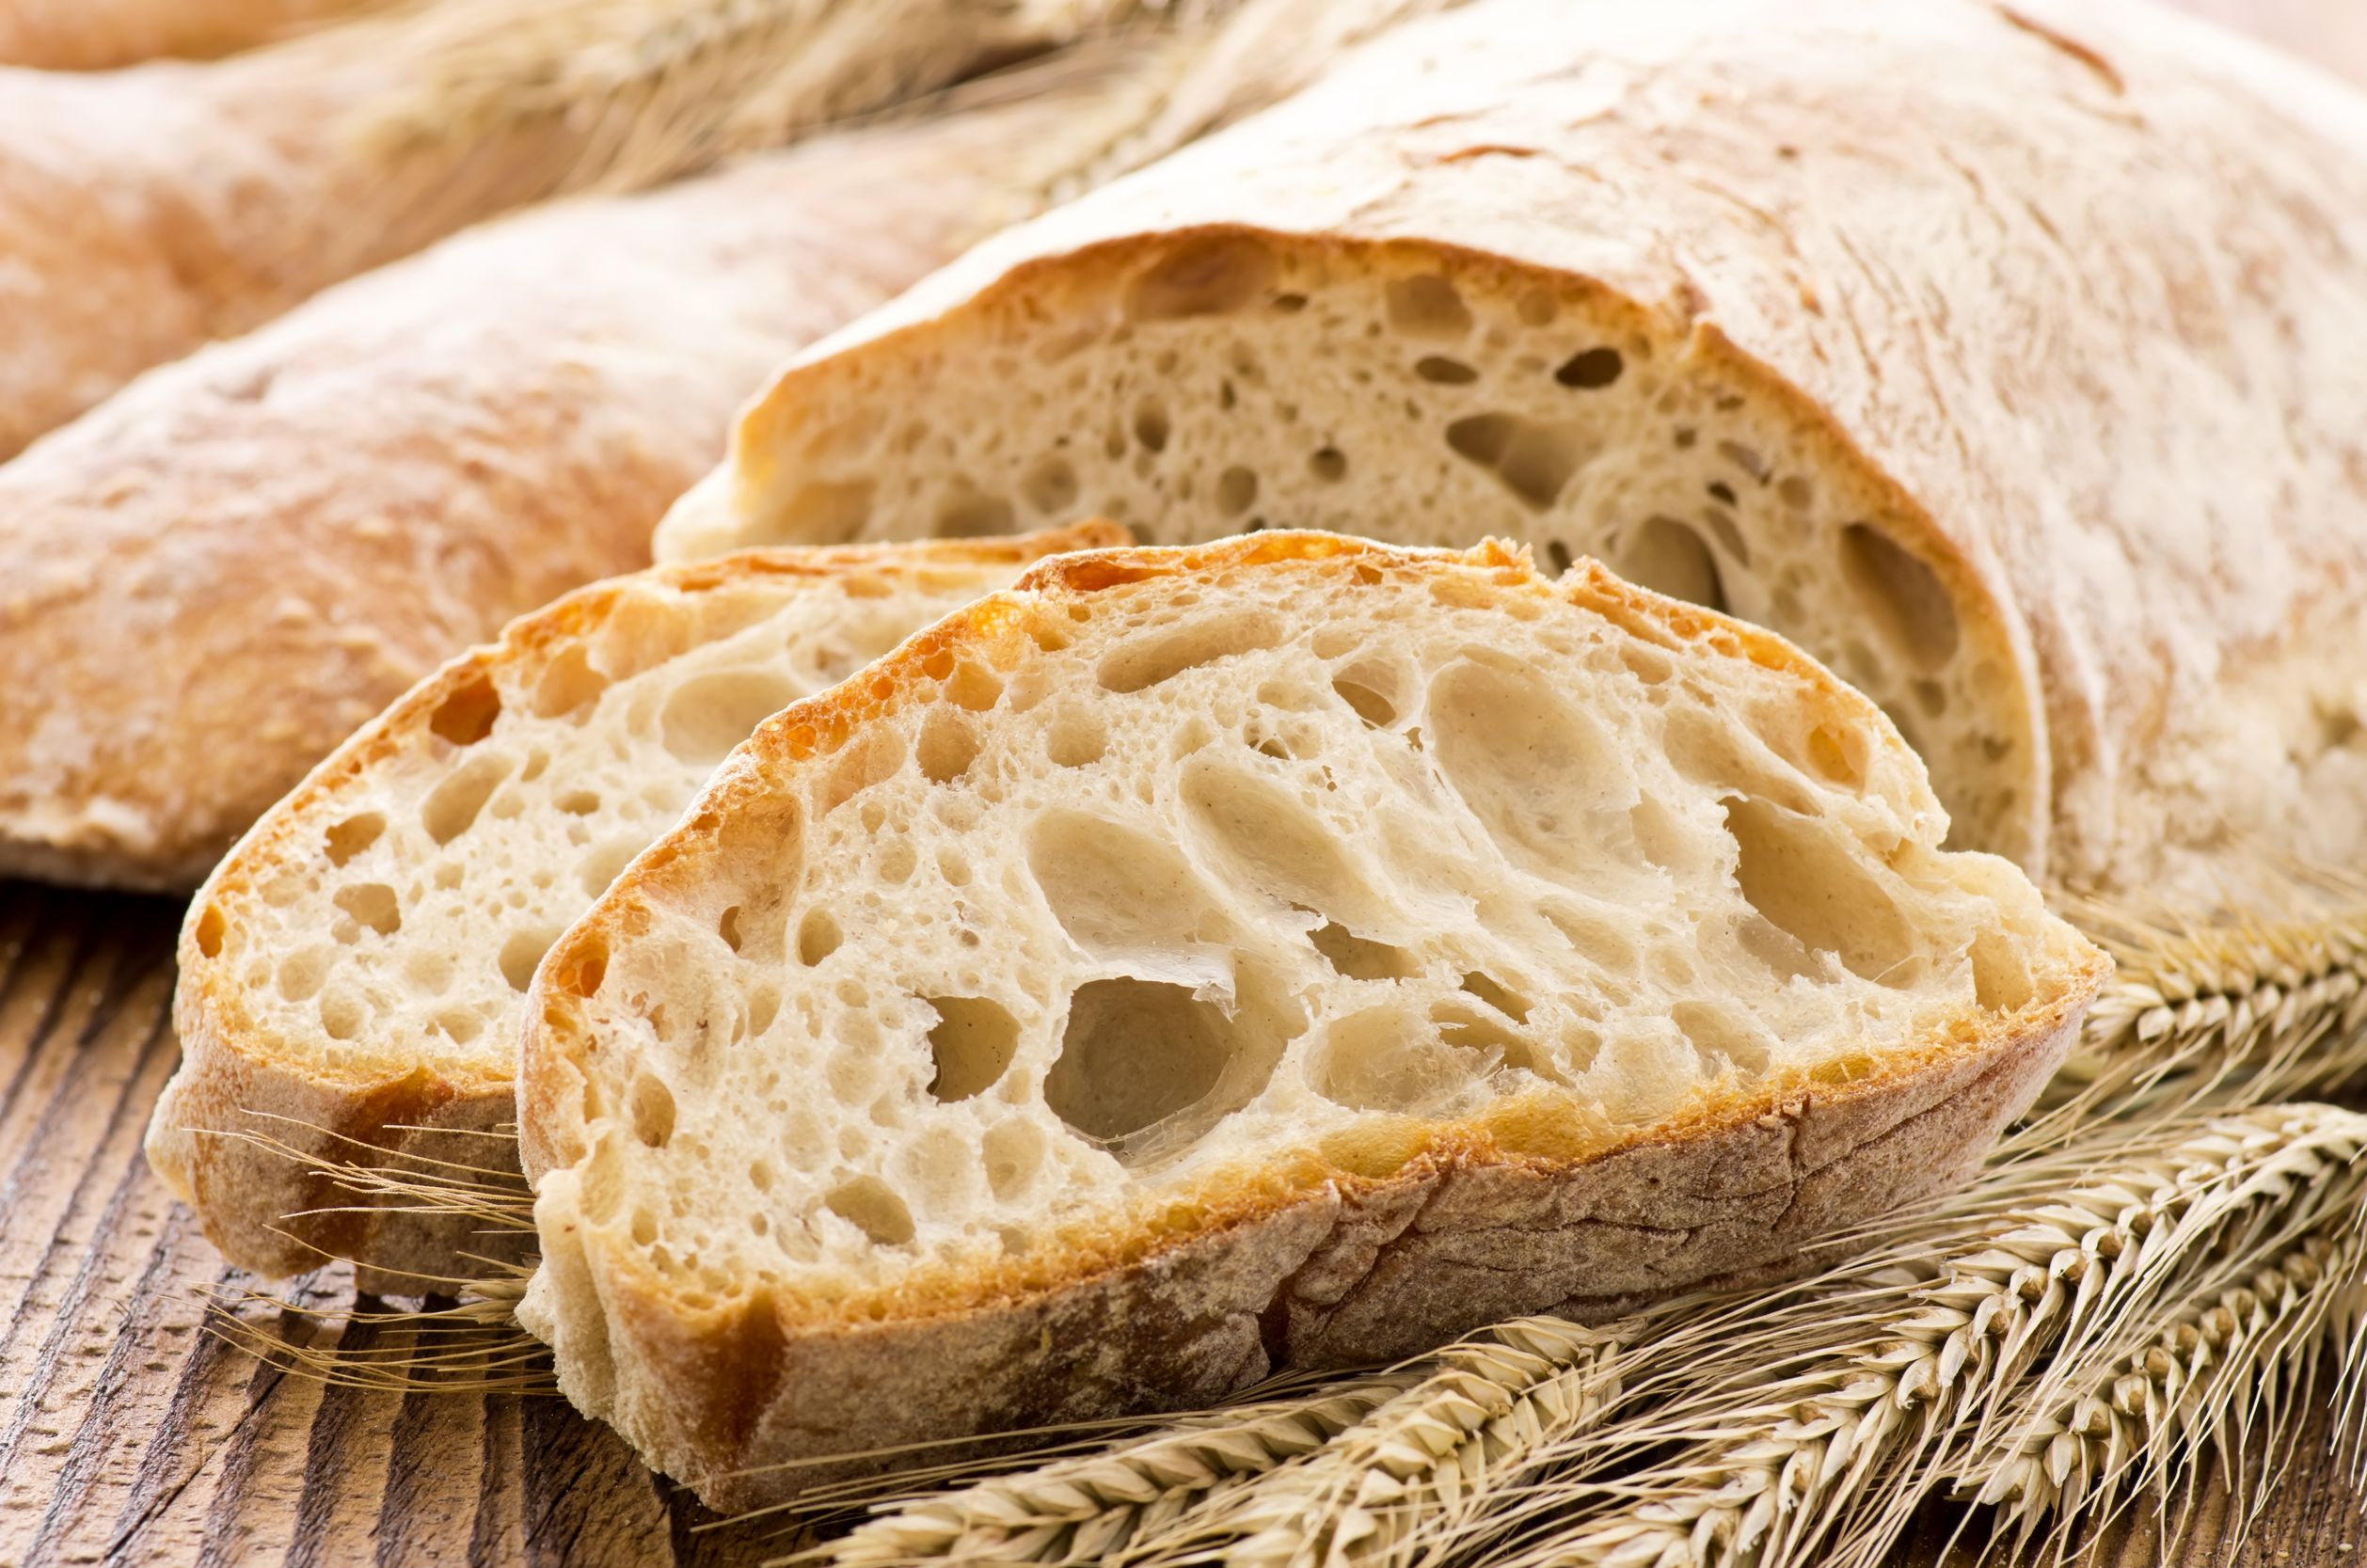
\includegraphics[width=\textwidth]{figures/bread.jpg}
	\end{column}
	\begin{column}{0.5\textwidth}
	\begin{itemize}
	\item Jesus used God as His basis for refuting Satan
	\item There is no objective morality without a God-provided standard
	\end{itemize}
	\end{column}
	\end{columns}
	
	\note{10:00}
	\note[item]{When God is `our' God, He sets the rules.}
	\note[item]{Jesus did not just quote any old verses from the Old Testament.}
	\note[item]{Every rebuttal was predicated on a respect for the greatness and authority of God.}
	\note[item]{Atheists, and indeed people in general, don't want an objective morality, until they become dissatisfied with their life}
	\note[item]{But, when we humble ourselves before God, we find refuge in the objective morality He provides.}
\end{frame}

\begin{frame}
	\frametitle{Love toward God is the foundation of eternal life}
	\framesubtitle{Luke 10:25-27}
	\begin{columns}
	\begin{column}{0.5\textwidth}
		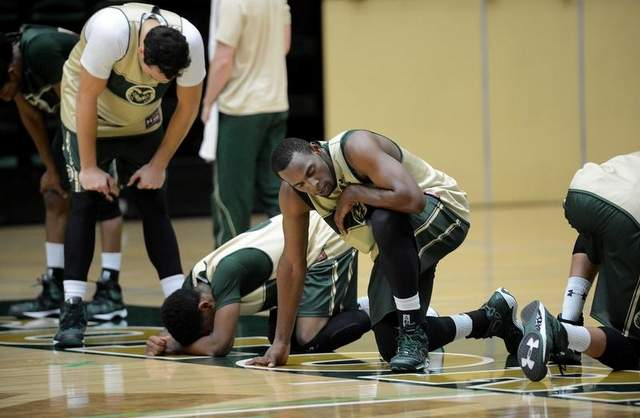
\includegraphics[width=\columnwidth]{figures/basketballRunning.jpg}
	\end{column}
	\begin{column}{0.5\textwidth}
		\begin{itemize}
			\item The main thing is to keep the main thing the main thing. -- {\footnotesize \emph{Steven Covey}}
			\item Sometimes we don't remember what giving all of ourselves looks like.
		\end{itemize}
	\end{column}
	\end{columns}
	\note{10:05}
	\note[item]{Loving God with all of ourselves is a `must have' for salvation.}
	\note[item]{We are not perfect.}
	\note[item]{In spite of that, though, we have to keep pushing.}
	\note[item]{Remember that we haven't given everything, yet.  We can always push to love God more.}
\end{frame}

\section{Review}

\begin{frame}
\frametitle{I will be their God}
\framesubtitle{God wants to be \emph{your} God}
\begin{columns}[c]
\begin{column}{0.3\textwidth}
	
\includegraphics[width=\columnwidth]{figures/uncleSam.jpg}
\end{column}
\begin{column}{0.7\textwidth}
	\begin{itemize}
		\item God is great and mighty
		\item God loves and blesses us.
		\item God shows Himself to man
		\item God's portrait is perfected in Jesus
		\item We meet Jesus in the Bible.  
		\item Respect for God can guide our lives
		\item Loving God is where salvation starts
	\end{itemize}
\end{column}
\end{columns}
\note{10:10}
\note[item]{Are you proud of being on God's team?}
\end{frame}

\end{document}


